\documentclass{article}
\usepackage[utf8]{inputenc}

\usepackage[a4paper,top=3cm,bottom=3cm,left=2cm,right=2cm,marginparwidth=1.75cm]{geometry}
\usepackage{svg}
\usepackage{tikz}
\usepackage{rotating}




%% Pour insérer le code
\usepackage[toc, page]{appendix}
\usepackage[french]{babel}
\usepackage{color}
\usepackage{fancyhdr}
\usepackage{fancyvrb}
\usepackage{fancyref}
\usepackage{listings}
\usepackage{lmodern}
\usepackage{lscape}
\usepackage{microtype}
\usepackage{subfigure}
\usepackage{verbatim}
\usepackage{mathrsfs}
\usepackage{epstopdf}
\usepackage{float}

\usepackage{eurosym}
\usepackage{cprotect}
\AddThinSpaceBeforeFootnotes
\FrenchFootnotes

\usepackage{hyperref}

\definecolor{monmauve}{rgb}{0.63,0.13,0.94}
\definecolor{monvert}{rgb}{0.13,0.55,0.13}
\lstset{
	columns=flexible,
	numbers = left,
	numberstyle = \small,
	stepnumber = 1,
	numbersep = 10pt,
	showspaces = false,
	showstringspaces=false,
	showtabs = false,
	tab = rightarrowfill,
	language = vhdl,
	basicstyle = \small,
	captionpos = b,
	linewidth= \linewidth,
	breaklines = true,
	commentstyle = \color{monvert}\usefont{T1}{pcr}{m}{sl},
	stringstyle = \color{monmauve},
	identifierstyle = \ttfamily,
	keywordstyle = \color{blue},
	frame=single,
	tabsize = 2
}






\title{Rapport de Projet : Tic Tac Toe}
\author{Grégoire Roumache - Alexandre Radoux \\ Joachim Paquay - Thomas Chavet}
\date{Avril 2018}

\begin{document}










\maketitle










\section{Introduction}





Nous avons décidé de faire le jeu tic tac toe (aussi appelé jeu du morpion) pour notre projet de Digital Electronics. Les deux joueurs doivent essayer d'aligner leur symbole respectif pour gagner sur une grille de 9 cases.

\begin{center} 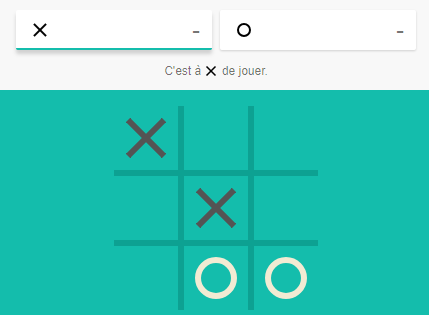
\includegraphics[width=0.5\textwidth]{images/TTT1.PNG} \end{center}










\section{Courte Présentation des Résultats Pratiques}





Pour adapter ce jeu à une forme électronique, nous avons utiliser des LED pour représenter chaque case et on utilise des couleurs au lieu des croix et des cercles.

\begin{center} 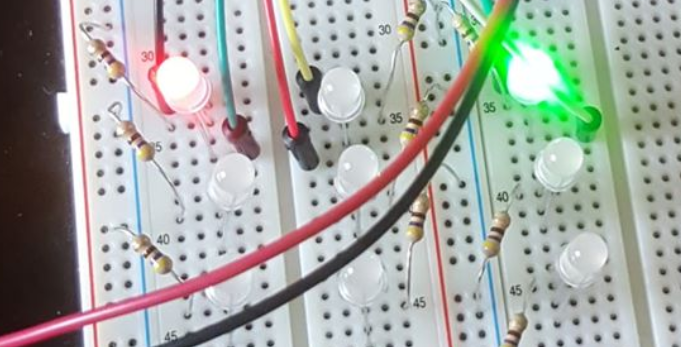
\includegraphics[width=0.5\textwidth]{images/TTT2.PNG} \end{center}

Pour savoir qui doit jouer, nous avons mis une LED supplémentaire qui indique si c'est au joueur rouge ou au vert de jouer. Ensuite, le joueur peut allumer la LED qu'il a sélectionné en appuyant sur le bouton B2.

\begin{center} 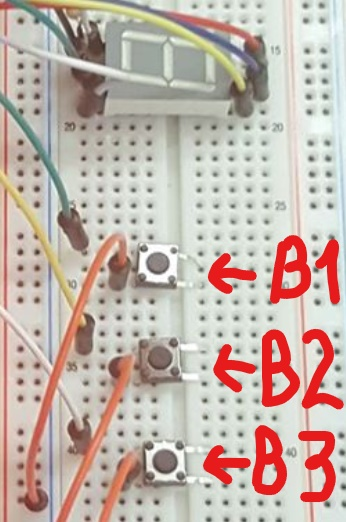
\includegraphics[width=0.4\textwidth]{images/TTT3_LI.jpg} \end{center}

Mais comment sélectionner cette LED ? En fait, en se servant du bouton B1, on peut incrémenter un compteur qui va de 0 à 8 et représente toutes les LED. Pour savoir où en est ce compteur, nous avons placé un afficheur 7-segments qui affiche la valeur de ce compteur.

\begin{center} \begin{tikzpicture}

\node(text) [rectangle, yshift = 1cm, xshift = 1.5cm] {\textbf{Numérotation des LED : }};
\node(0) [rectangle, draw=black, minimum width=1cm, minimum height=1cm, fill=red!30, rounded corners] {\textbf{0}};
\node(1) [rectangle, draw=black, minimum width=1cm, minimum height=1cm, rounded corners, xshift = 1.5cm] {\textbf{1}};
\node(2) [rectangle, draw=black, minimum width=1cm, minimum height=1cm, fill=green!30, rounded corners, xshift = 3cm] {\textbf{2}};
\node(3) [rectangle, draw=black, minimum width=1cm, minimum height=1cm, rounded corners, xshift = 0cm, yshift = -1.5cm] {\textbf{3}};
\node(4) [rectangle, draw=black, minimum width=1cm, minimum height=1cm, rounded corners, fill=red!30, xshift = 1.5cm, yshift = -1.5cm] {\textbf{4}};
\node(5) [rectangle, draw=black, minimum width=1cm, minimum height=1cm, rounded corners, xshift = 3cm, yshift = -1.5cm] {\textbf{5}};
\node(6) [rectangle, draw=black, minimum width=1cm, minimum height=1cm, rounded corners, fill=green!30, xshift = 0cm, yshift = -3cm] {\textbf{6}};
\node(7) [rectangle, draw=black, minimum width=1cm, minimum height=1cm, rounded corners, xshift = 1.5cm, yshift = -3cm] {\textbf{7}};
\node(8) [rectangle, draw=black, minimum width=1cm, minimum height=1cm, rounded corners, xshift = 3cm, yshift = -3cm] {\textbf{8}};

\end{tikzpicture} \end{center}

Quant au bouton B3, il sert à lancer une nouvelle partie en cas d'égalité. Mais dans le cas d'une victoire, toutes les LED s'allument de la même couleur (celle du gagnant) pour montrer qui a gagné.

\begin{center}
\begin{figure}[h!]
    \centering
    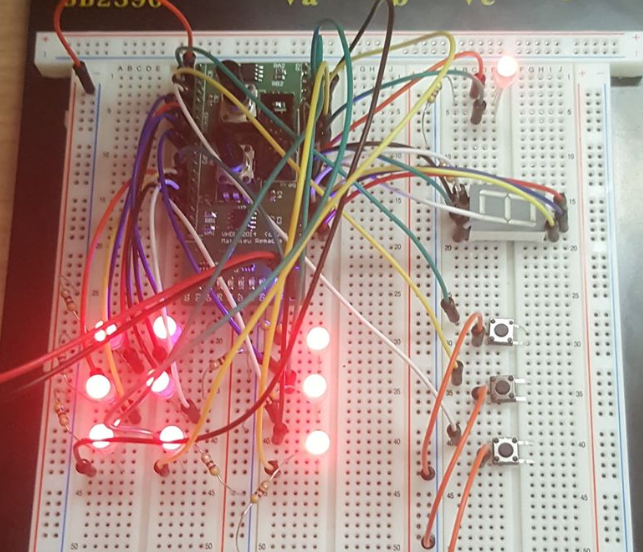
\includegraphics[width=0.65\textwidth]{images/TTT4.PNG}
    \caption{Exemple : Victoire Rouge}
    \label{fig:my_label}
\end{figure}
\end{center}










\newpage










\section{Explication des Variables du Code VHDL}





\begin{enumerate}





%% Entrées
\item Comme entrées du système, nous avons : 
\begin{itemize}
\item Les 3 boutons \texttt{button0}, \texttt{button1} et \texttt{button3} qui correspondent respectivement aux boutons surnommés B1, B2 et B3 dans la section du rapport ci-dessus.
\item L'horloge \texttt{clk} qui sert à filtrer les signaux venant des boutons, c-à-d qu'on veut éviter que lorsqu'on appuie sur le bouton pour incrémenter le compteur (ex : compteur = 5 $ \longrightarrow $ compteur = 6)  les rebonds n'augmente le compteur d'une valeur aléatoire (ex : compteur = 5 $ \longrightarrow $ compteur = 9).
\end{itemize}





%% Sorties
\item Les sorties du systèmes sont : 
\begin{itemize}
\item \texttt{ledTurnGreen} \& \texttt{ledTurnRed}, elles désignent quel joueur doit jouer en allumant la LED en haut à gauche de la figure 1.
\item Les vecteurs \texttt{ledGreen} \& \texttt{ledRed} qui sont de taille 9 et donne leur couleur aux LED en bas à gauche de la figure 1.
\item \texttt{seg1}, \texttt{seg2}, ... , \texttt{seg7} qui allument les segments de l'afficheur 7-segments.
\begin{center} \begin{tikzpicture}

\node (seg1) [rectangle, rounded corners, draw = black, text width = 1.5cm, text centered, fill=red!30] {\texttt{seg1}};
\node (seg2) [rectangle, rounded corners, draw = black, text width = 1.5cm, text centered, xshift = -1.2cm, yshift = 1.2cm, rotate = 90] {\texttt{seg2}};
\node (seg3) [rectangle, rounded corners, draw = black, text width = 1.5cm, text centered, yshift = 2.4cm, fill=red!30] {\texttt{seg3}};
\node (seg4) [rectangle, rounded corners, draw = black, text width = 1.5cm, text centered, xshift = 1.2cm, yshift = 1.2cm, rotate = 90, fill=red!30] {\texttt{seg4}};
\node (seg5) [rectangle, rounded corners, draw = black, text width = 1.5cm, text centered, xshift = -1.2cm, yshift = -1.2cm, rotate = 90, fill=red!30] {\texttt{seg5}};
\node (seg6) [rectangle, rounded corners, draw = black, text width = 1.5cm, text centered, yshift = -2.4cm, fill=red!30] {\texttt{seg6}};
\node (seg7) [rectangle, rounded corners, draw = black, text width = 1.5cm, text centered, xshift = 1.2cm, yshift = -1.2cm, rotate = 90] {\texttt{seg7}};

\end{tikzpicture} \end{center}
\end{itemize}





%% Variables
\item Les variables internes au système sont : 
\begin{itemize}
\item Les vecteurs \texttt{ledVert} \& \texttt{ledRouge} qui sont associés aux vecteurs \texttt{ledGreen} \& \texttt{ledRed} qui, eux, sont en sortie.
\item \texttt{TourRouge} qui vaut 1 si c'est au tour du joueur rouge de jouer et qui vaut 0 si c'est au joueur vert de jouer.
\item \texttt{VictoireRouge} qui vaut 1 lorsque le joueur rouge gagne et son homologue \texttt{VictoireVert} qui vaut évidemment 1 en cas de victoire du joueur vert.
\item La variable \texttt{ledSelect} qui fait office de compteur pour sélectionner la LED que le joueur veut allumer.
\item Les variables \texttt{SUPERcounter0}, \texttt{SUPERcounter1}, \texttt{SUPERcounter2} qui servent à éviter les rebonds. Il y en a un pour chaque bouton et elles sont expliquées plus en détail dans la section suivante.
\end{itemize}



\end{enumerate}










\section{Dispositif anti-rebonds}





Ci-dessous se trouve le code utilisé pour empêcher les rebonds de créer des problèmes avec le compteur qui sert à sélectionner les LED.

\begin{lstlisting}
	-- Utilisation du button0 pour selectionner la led
			if(button0 = '0') then
				SUPERCOUNTER0 <= SUPERcounter0 + 1;
			else
				SUPERcounter0 <= 0;
			end if;

			if(SUPERcounter0 = 250) then

				ledSelect <= ledSelect + 1;
				if(ledSelect = 9) then
					ledSelect <= 0;
				end if;

			end if;
\end{lstlisting}

À l'origine, nous avions remarqué un problème : lorsque le joueur voulait choisir la LED à allumer, il ne pouvait pas la sélectionner correctement car le compteur augmentait de manière aléatoire... Pour résoudre ce problème, nous avons utilisé l'horloge interne de la CPLD (\texttt{clk}). À chaque fois que la condition \texttt{rising\_edge( clk )} est vraie, le code va vérifier si le joueur appuie sur le boutton B1 (= variable interne \texttt{button0}) ce qui fait que \texttt{button0} = '0'. Si c'est le cas, alors la variable \texttt{SUPERcounter0} est incrémentée, et lorsque \texttt{SUPERcounter0} vaut 250, on estime qu'il n'est pas possible que ça soit un hasard dû aux rebonds mais que l'utilisateur veut vraiment augmenter le compteur (c-à-d incrémenter \texttt{ledSelect}).

Si la variable \texttt{SUPERcounter0} n'atteint pas la valeur 250 et que le bouton prend la valeur 1 alors, le programme "comprends" que c'est dû à un/des rebonds et qu'il ne faut en fait pas augmenter le compteur. La variable \texttt{SUPERcounter0} est donc remise à 0.

Le seul inconvénient de cette approche est qu'il faut appuyer un certain temps sur un bouton pour que le programme le prenne en compte. Ce temps d'attente est réglable grâce au potentiomètre présent sur la CPLD. Dans notre cas, le temps d'attente va d'environ 0.5 sec à 5 sec.

L'avantage de cette approche est la très faible probabilité que les rebonds enclenchent l'activation d'un bouton. En effet, puisqu'il faut que le compteur (\texttt{SUPERcounter0}) augmente jusqu'à 250, il faudrait que \texttt{button0} prenne la valeur '1' 250 fois d'affilée. Or, il y a 50\% de chance qu'elle prenne cette valeur (observation expérimentale) et donc, Il y a une chance sur $ 2^{250} \simeq 10^{75} $ que cela arrive.










\newpage










\section{Tests}





Voici un des tests que nous avons effectués.

\begin{center} 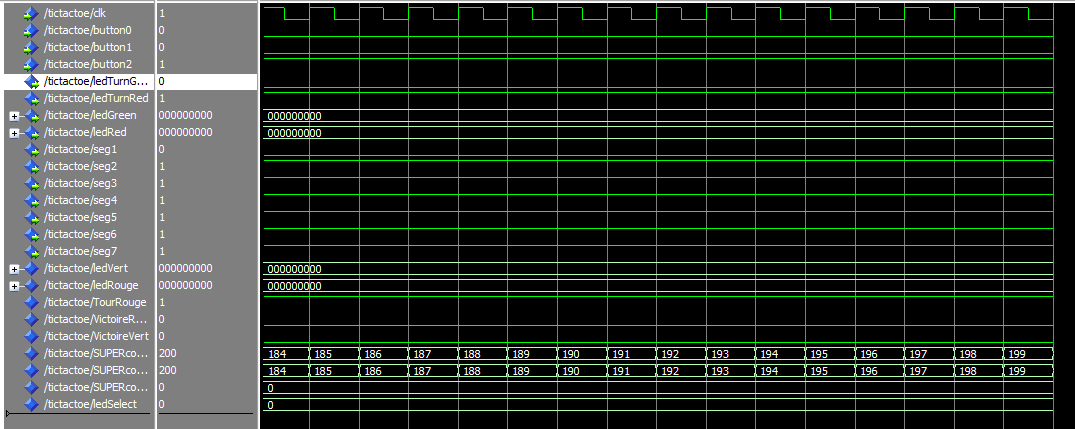
\includegraphics[width=0.75\textwidth]{images/test1.PNG} \end{center}































\appendix










\section*{Annexes}










\subsection*{A. Code VHDL de Tic Tac Toe}

\lstinputlisting{TicTacToe.vhd}












\end{document}
